\documentclass{myassignment}
\usepackage{multicol}

\courselabel{MAT1100}
\coursetitle{Kalkulus}
\exercisesheet{Oblig 1}{Obligatorisk oppgave 1 av 2}



\begin{document}
	\begin{problem}
		Skriv det komplekse tallet $z=\frac{6}{\sqrt{3}+3i}$ først på formen $a+ib$ også på polarformen $re^{i\theta}$.
	\end{problem}

		\begin{multicols}{2}
			\begin{answer}
				\begin{align*}
					z &= \frac{6}{\sqrt{3}+3i} \\[0.4em]
					z &= \frac{2}{\sqrt{\frac{1}{3}}+i} \\[0.4em]
					z &= \frac{2\times(\sqrt{\frac{1}{3}}-i)}{(\sqrt{\frac{1}{3}}+i)\times(\sqrt{\frac{1}{3}}-i)} \\[0.4em]
					z &= \frac{2\times(\sqrt{\frac{1}{3}}-i)}{\frac{1}{3}-i^2} \\[0.4em]
					z &= \frac{2\times(\sqrt{\frac{1}{3}}-i)}{\frac{4}{3}} \\[0.4em]
					z &= \frac{3\times(\sqrt{\frac{1}{3}}-i)}{2} \\[0.4em]
					z &= \frac{\sqrt{3}}{2} - \frac{3}{2}i
				\end{align*}
				\vspace*{\fill}
			\end{answer}

				\vspace*{2em}
				\begin{center}
				Using $z = \frac{\sqrt{3}}{2} - \frac{3}{2}i$:

				%\raisebox{-.5\height}{
				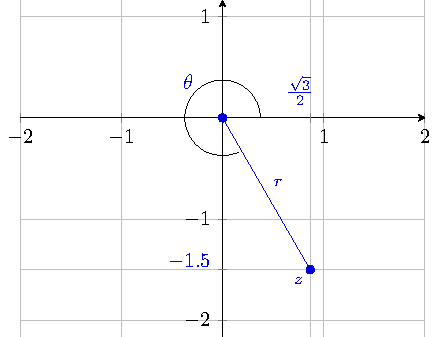
\includegraphics[scale=1]{graphact1.pdf}
				%}
				\end{center}
			\columnbreak

			\begin{answer}
				\textit{\hspace*{2em}\small With Pythagora's Theorem}
				\begin{align*}
					r &= \sqrt{(\frac{\sqrt{3}}{2})^2 +(\frac{3}{2})^2}\\
					r &= \sqrt{\frac{3}{4} + \frac{9}{4}} \\
					r &= \sqrt{3}
				\end{align*}
				\blackqed
				\vspace*{-1em}

				\textit{\hspace*{2em}\small By the laws of trigonometry}
				\begin{align*}
					\theta' &:= 2\pi - \theta\\[1em]
					\sin(\theta') &= \frac{-1.5}{\sqrt{3}} \\
					\theta' &= \arcsin(\frac{-1.5\sqrt{3}}{3}) \\[0.5em]
					\theta' &= \arcsin(\frac{-\sqrt{3}}{2}) \\[0.5em]
					\theta' &= -\frac{\pi}{3} \equiv \frac{5\pi}{3} \\[0.5em]
					\therefore \theta  &= \frac{\pi}{3} \\
				\end{align*}
				\blackqed
				\textit{\small \hspace*{3em}And since $z$ is in the fourth quadrant, as $Re(z)>0 \land Im(z)<0$ we know to use $\theta'$:}
				\begin{align*}
					r: \sqrt{3} \land \theta: \frac{5\pi}{3} \therefore z = \sqrt{3}e^{\frac{-i\pi}{3}} \equiv \sqrt{3}e^{\frac{5i\pi}{3}}
				\end{align*}
			\end{answer}
		\end{multicols}
		\pagebreak


	\begin{problem}
		Finn de to løsningene til likningen $w^2 - w + 1 = 0$, og bruk disse til å finne alle komplekse løsninger til likningen $z^4 - z^2 + 1 = 0$. Gi en faktorisering av $z^4 - z^2 + 1$, først i komplekse førstegradspolynomer og så i reelle andregradspolynomer.
	\end{problem}

	Assuming $cis(x) \equiv cos(x) + i\cdot sin(x)$, and $i^2=-1$.
	\begin{answer}
		\begin{eqnarray}
			&a = 1, b = -1, c = 1 \\
			&w = \frac{1\pm\sqrt{1-4}}{2} = \frac{1}{2}\pm\frac{\sqrt{3}}{2}i\\
		\end{eqnarray}
		\text{With $t = z^2$}:\\
		\begin{eqnarray}
			&z^4 - z^2 + 1 = t^2-t^2+1 = 0\\
			&t = {\frac{1}{2}\pm\frac{\sqrt{3}}{2}i}\\
		\end{eqnarray}
		\text{With $t_0 = \frac{1}{2}+\frac{\sqrt{3}}{2}i = cis(\frac{\pi}{3})$:}\\
		\begin{eqnarray}
			&\sqrt{cis(\frac{\pi}{3})}^4 - \sqrt{cis(\frac{\pi}{3})}^2 + 1 = 0\\
			&cis^2(\frac{\pi}{3}) - cis(\frac{\pi}{3}) + 1 = 0\\
		\end{eqnarray}
		With De Moivres formula:
		\begin{eqnarray}
			&cis(\frac{2\pi}{3}) - cis(\frac{\pi}{3}) + 1 = 0\\
			&cos(\frac{2\pi}{3}) + i\cdot sin(\frac{2\pi}{3}) - cos(\frac{\pi}{3}) - i\cdot sin(\frac{\pi}{3}) + 1 = 0\\
			&-\frac{1}{2} + \frac{\sqrt{3}}{2}i - \frac{1}{2} - \frac{\sqrt{3}}{2} i + 1 = 0\\
			&-\frac{1}{2} - \frac{1}{2} + 1 = 0\\
			&-1 + 1 = 0\\
		\end{eqnarray}
		Therefore, $z = t_0^{\frac{1}{2}} = cis^{\frac{1}{2}}(\frac{\pi}{3}) = cis(\frac{\pi}{6})$ is a root $z_0$.\\
		By the complex conjugate root theorem, $z=t_1^{\frac{1}{2}}=cis^{\frac{1}{2}}(-\frac{\pi}{3})=cis(-\frac{\pi}{6})$ is a root $z_0'$.\\
	\end{answer}


	\pagebreak
	\begin{problem}
		Finn grensene $\lim_{n \rightarrow \infty}\frac{3n + 2}{\sqrt{4n^2 - 1}}$ og $\lim_{n\rightarrow\infty}(\sqrt{n^2 - 5n} - n)$.
	\end{problem}

	\begin{multicols}{2}
		\begin{answer}
			\begin{align*}
				\lim_{n \rightarrow \infty} &\frac{3n + 2}{\sqrt{4n^2 - 1}} = \\[1em]
				\lim_{n \rightarrow \infty} &\frac{(3n + 2)\frac{1}{n}}{\sqrt{4n^2 -1}\frac{1}{n}} = \\[1em]
				\lim_{n \rightarrow \infty} &\frac{3 + \frac{2}{n}}{\sqrt{\frac{4n^2 -1}{n^2}}} = \\[1em]
				\lim_{n \rightarrow \infty} &\frac{3 + \frac{2}{n}}{\sqrt{4 - \frac{1}{n^2}}} = \\[1em]
				&\frac{3 + \not{0}}{\sqrt{4 -\not{0}}} = \\[1em]
				&\frac{3}{2}
			\end{align*}
		\end{answer}

		\columnbreak
		\begin{answer}
			\begin{align*}
				\lim_{n\rightarrow\infty}&(\sqrt{n^2 - 5n} - n)\\[1em]
				\lim_{n\rightarrow\infty}&\frac{(\sqrt{n^2 - 5n} - n)(\sqrt{n^2 - 5n} + n)}{\sqrt{n^2 - 5n}+n }\\[1em]
				\lim_{n\rightarrow\infty}&\frac{n^2 - 5n - n^2}{\sqrt{n^2 - 5n}+n }\\[1em]
				\lim_{n\rightarrow\infty}&\frac{-5n}{\sqrt{n^2 - 5n}+n }\\[1em]
				\lim_{n\rightarrow\infty}&\frac{-5}{\sqrt{1 - \frac{5}{n}}+1 }\\[1em]
				&\frac{-5}{\sqrt{1 - \not{0}}+1 }\\[1em]
				&\frac{-5}{2}
			\end{align*}
		\end{answer}

	\end{multicols}

	\newpage
	\begin{problem}
		Finn de komplekse tallene $z$ som oppfyller likningen $2|z - 1|=|z - 4|$ og skisser løsningsmengden i det komplekse planet.(Hint: Sett inn $z = x + iy$ og finn en polynomlikning $ix$ og $y$ forløsningsmengden.)
	\end{problem}

	\begin{answer}
		\begin{multicols}{2}
			\begin{align*}
				% since |a|=sqrt(a^2+b^2)
				2|z-1| &= |z-4| \equiv \\[2em]
				4|x+iy-1| &= |x+iy-4|\\[1em]
				4((x-1)^2+(y)^2) &= (x-4)^2+(y)^2 \\[1em]
				4(x-1)^2+4y^2 &= x^2-8x+16+y^2 \\[1em]
				4(x^2-2x+1)+4y^2 &= x^2-8x+16+y^2 \\[1em]
				4x^2-8x+4 + 4y^2 &= x^2-8x+16+y^2 \\[1em]
				3x^2 + 3y^2 &= 12 \\[1em]
				y^2 &= 4 - x^2 \\[1em]
				y &= \sqrt{4 - x^2}\\[1em]
				\therefore Im(z) &= \pm\sqrt{4 - Re(z)^2}, \exists z \forall \{x \in Re(z) | -2 < x <2 \} \\[1em]
			\end{align*}
		\columnbreak
		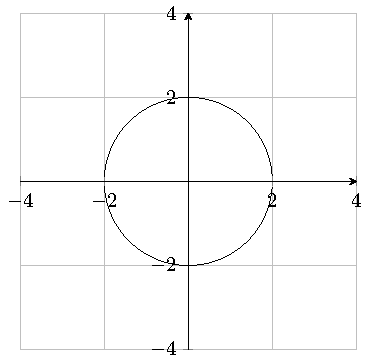
\includegraphics{graphact4}

		\end{multicols}
	\end{answer}


	\begin{problem}
		En følge $\{ a_n \}$ er definert ved $a_1 = 3, a_n + 1 = 3\sqrt{a_n}$ for $n \geq 1$.Vis at $a_n < 9$ og at $a_n+1 > a_n$ for alle $n$. Forklar hvorfor følgen konvergerer og finn $\lim_{n \rightarrow \infty}{a_n}$
	\end{problem}

	\begin{answer}

	\end{answer}.
\end{document}